\documentclass[a4paper,12pt,twoside]{article}

\usepackage[a4paper, inner=2cm, outer=2cm,top=2cm, bottom=2cm]{geometry}
\usepackage[utf8]{inputenc}
\usepackage[portuges]{babel}
\usepackage{aeguill}
\usepackage{indentfirst}
\usepackage{xcolor}
\usepackage{graphicx}
\usepackage{titlesec}
\usepackage{titling}
\usepackage{wrapfig}
\usepackage{caption}
\usepackage{subcaption}
\usepackage{enumitem}
\usepackage{amsmath}
\usepackage{amssymb}
\usepackage{color}
\usepackage{setspace}
\usepackage{titlesec}
\usepackage{listings}
\usepackage{pdfpages}
\usepackage[autostyle]{csquotes}

\input{/home/lucas/docs/latex/lstset}

\usepackage{fancyhdr} %pagenumber top right
\fancyhf{}
\fancyheadoffset{0cm}
\renewcommand{\headrulewidth}{0pt}
\renewcommand{\footrulewidth}{0pt}
\fancyhead[R]{\thepage}
\fancypagestyle{plain}{%
    \fancyhf{}%
    \fancyhead[R]{\thepage}%
}

\renewcommand*{\thepage}{\footnotesize\arabic{page}}


% \titleformat{\section}
% {\normalfont\fontsize{12}{15}\bfseries}{\thesection}{1em}{}
% \titleformat{\subsection}
% {\normalfont\fontsize{12}{15}\bfseries}{\thesubsection}{1em}{}
% \titleformat{\subsubsection}
% {\normalfont\fontsize{12}{15}\bfseries}{\thesubsubsection}{1em}{}

\input{/home/lucas/docs/latex/hyper}

\hypersetup{
    pdftitle={Detecção e Reconhecimento de Peças e Posições
    em um Tabuleiro de Xadrez},
    pdfkeywords={Xadrez} {Zerdax} {Machine Learning} {Computer Vision},
    % pdftitle={My title},          % title
    % pdfsubject={Subject},         % subject of the document
    % pdfproducer={Producer},       % producer of the document
    % pdfkeywords={keyword1} {key2} % list of keywords
}

\usepackage[backend=biber,sorting=none]{biblatex}
\addbibresource{refs.bib}

\newenvironment{boldenv}
{\bfseries}
{}
\onehalfspacing

\title{Detecção e Reconhecimento de Peças e Posições em um Tabuleiro de Xadrez}
\author{Alexandre Ferreira de Carvalho Filho}
\author{Lucas Budde Mior}
\author{Vitor Dias Javornik}

\begin{document}
\begin{titlepage}
    \large
    \begin{center}
        \begin{boldenv}
            UNIVERSIDADE FEDERAL DE SANTA CATARINA \\
            DEPARTAMENTO DE ENGENHARIA ELÉTRICA \\
            CURSO DE ENGENHARIA ELÉTRICA \\
            \vspace*{2cm}

            \vspace*{\fill}
            Detecção e Reconhecimento de Peças e Posições \\
            em um Tabuleiro de Xadrez \\
            \vspace*{1cm}
            Proposta de Projeto \\
            \vspace*{1cm}
            EEL7815 - Projeto Nível I em Cont e Proc de Sinais I \\
            EEL7513 – Tópicos Avançados Em Controle Processos De Sinais IV
            \vspace*{\fill}

            Alexandre Ferreira de Carvalho Filho \\
            Lucas Budde Mior \\
            Vitor Dias Javornik \\
            \vspace{0.5cm}
            Professores: \\
            Danilo Silva (EEL7513) \\
            Joceli Mayer (EEL7815)

            \vfill

            Florianópolis, 30 de Junho de 2022.
        \end{boldenv}
    \end{center}
\end{titlepage}
\renewcommand{\contentsname}{Sumário}

\newgeometry{a4paper, inner=3cm, outer=2cm}
\pagestyle{empty}
\addtocontents{toc}{\protect\thispagestyle{empty}}
\tableofcontents
\newpage

% \section*{Resumo} %com 3 ou 4 palavras chave
% blablabla


\pagestyle{plain}
\section{Introdução} % revisão bibliográfica, justificativa e objetivos
Identificar, através de uma foto,
peças de xadrez e sua localização em um tabuleiro não é tarefa fácil, nem rápida.
Mesmo para humanos, de acordo com a distância e ângulo com a qual se vê um tabuleiro,
é possível se confundir.

Porém, esta é uma atividade recorrente entre a comunidade enxadrística.
Por vezes, durante uma partida,
é interessante gravar uma determinada posição crítica para posterior avaliação
(possivelmente, utilizando computadores).
Durante torneios, as transmissões precisam, de alguma forma,
conhecer a posição atual para informar aos narradores e telespectadores.
Além disso, torneios oficiais (especialmente aqueles realizados em países mais pobres como o Brasil),
nem sempre contam com um tabuleiro capaz de determinar a localização de cada peça automaticamente.
Sem este tabuleiro, é necessário inferir a posição manualmente.

Este projeto propõe uma solução para esses problemas.
O programa seria muito útil se utilizado, por exemplo, em um smartphone,
onde o usuário poderia utilizar a saída
(notação FEN da posição) como entrada de um programa de avaliação de melhores lances,
como o Stockfish, por exemplo, ou mesmo realizar pequenos ajustes devido a erros de predição do modelo.

\vspace{0.3in}
\setlength{\parindent}{0in}
\textbf{Palavras Chave:} Xadrez, Zerdax, Machine Learning, Computer Vision.

\setlength{\parindent}{0.4in}

\begin{figure}[h!]
    \centering
    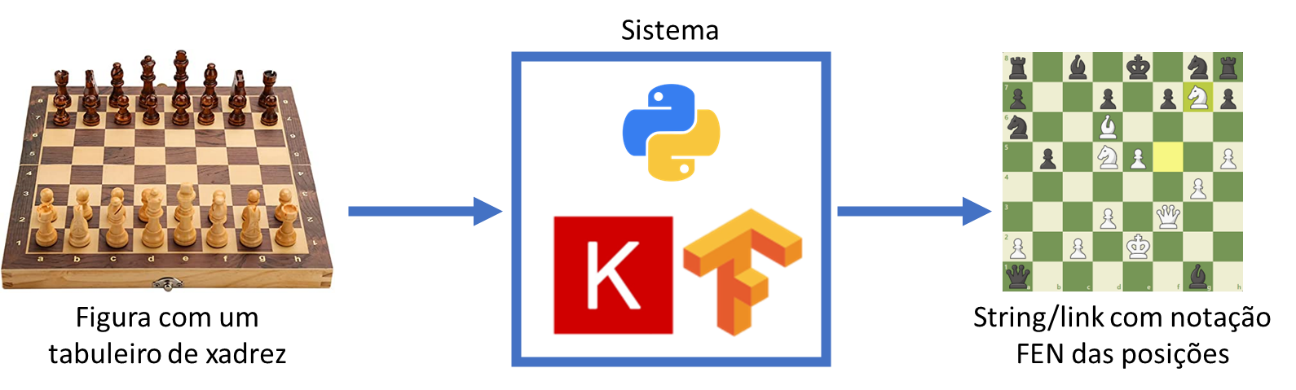
\includegraphics[width=\linewidth]{fig/sistema.png}
    \caption{Esquemático do Sistema}
    \label{fig:sistema}
\end{figure}

\vspace{0.5in}
\newpage

\section{Objetivos}
A partir da importação de uma foto nas seguintes condições:

\begin{enumerate}
    \item{O tabuleiro ocupando a maior parte da foto}
    \item{A ângulo da câmera em aproximadamente 30° do chão,
          o suficiente para visualizar o perfil das peças, sem que haja muita sobreposição}
    \item{Peças de plástico ou madeira, ambos com um nível baixo ou moderado de reflexão no tabuleiro,
          de acordo aos datasets em posse.}
\end{enumerate}

O sistema deverá ser capaz de reconhecer e segmentar a superfície do tabuleiro,
segmentar as casas deste, detectar peças,
então classificá-las com o uso de redes neurais convolucionais profundas.
Após cruzar as peças com suas respectivas casas,
o programa fornecerá em notação FEN uma string ou uma URL da partida de xadrez no lichess.

Três desafios nortearão o desenvolvimento do projeto:

\begin{enumerate}
    \item{Detecção das bordas}
    \item{Detecção das casas}
    \item{Detecção das peças}
\end{enumerate}

As primeiras duas etapas serão atingidas por técnicas de Visão Computacional (CV),
enquanto a última, por meio de machine learning.

\subsection{Computer Vision}

A primeira coisa a ser feita com as imagens fornecidas ao sistema,
seja para treino ou teste, é filtrá-las para garantir seu melhor aproveitamento.
A princípio, a segmentação do tabuleiro,
determinação das cores (das casas e peças) e determinação da localização das casas e posição das peças
será feita utilizando técnicas tradicionais de processamento de imagem,
como equalização de histograma, detecção de borda, threshold, morfologia etc.

\subsubsection{Segmentação do Tabuleiro}
Uma abordagem possível para esse problema consiste no uso das seguintes técnicas:
\begin{itemize}
    \item{Utilizar algoritmo de Canny (ver figura \ref{fig:detector}) para detectar bordas}
    \item{Obter cantos do tabuleiro e corrigir perspectiva}
\end{itemize}

\begin{figure}[h!]
\centering
  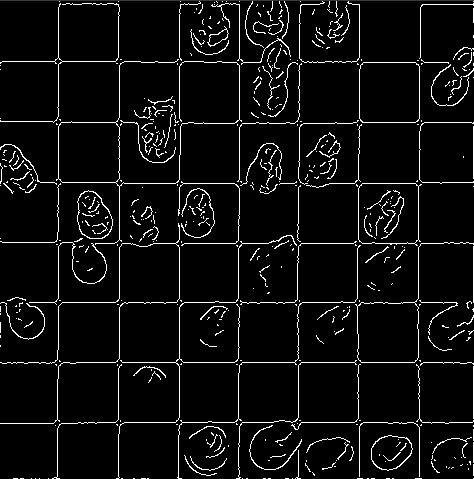
\includegraphics[width=0.6\linewidth]{fig/detector.png}
\caption{Exemplo de detector de bordas de Canny}
\label{fig:detector}
\end{figure}

\subsubsection{Determinação da localização das casas}
Para dividir o tabuleiro em suas 64 casas,
é possível utilizar a transformada \textit{Hough} para detectar intersecções das linhas do passo anterior.
A partir da seleção das intersecções que formam um arranjo de 8 fileiras de 8 quadrados,
pode-se obter a localização das casas.

\subsubsection{Determinação das cores das casas e peças}
Será necessário escolher um limiar de separação.
Para isso, será realizada a filtragem da imagem
(provavelmente usando o filtro mediano) para remover pontos ``fora da curva".
A identificação da cor da casa e peça deve ser escolhida 
de acordo com os 4 níveis de amplitude esperados 
(casa branca, casa preta, peça branca, peça preta).

O reflexo causado por luzes incidentes nas peças pode atrapalhar esse processo,
portanto a eficácia da filtragem é importante.
Uma técnica adicional que pode ser utilizada é obter a cor média
da região da peça (se for desenvolvido um algoritmo robusto de segmentação
da peça).

\subsubsection{Segmentação de Região com Peça}
Essa parte envolve uma combinação dos resultados de localização das casas,
com técnicas de reconhecimento de objetos.
Pode-se usar técnicas de morfologia sobre as segmentações das casas,
e combinar esse processo com técnicas de aprendizado de máquina que também reconhecem objetos.

O objetivo principal da etapa de CV é obter as melhores segmentações a serem usadas pela rede neural
que será encarregada de reconhecer as peças.
Inclusive, a ser definido, 
existe a possibilidade de o reconhecimento de peças ser feito utilizando apenas a forma das peças,
desconsiderando as cores.

Esta fatia do projeto será elaborada na disciplina de Projeto Nível I em Controle e Processamento de Sinais,
com o apoio do professor Joceli Meyer.

\subsection{Machine Learning}

\subsubsection{Datasets}

Foi dada atenção especial ao conjunto de dados,
pois boa parte do resultado deste projeto dependerá deste.
Após vasta pesquisa no Google, foram encontrados alguns datasets interessantes:

\begin{enumerate}
    \item{Dataset of Rendered Chess Game State Images –
          \textbf{4888} imagens renderizadas, com informações ricas em json sobre: bordas do tabuleiro, nome das peças, posições, ângulo de câmera, iluminação etc.
      Disponível em: \url{https://osf.io/xf3ka/}}\label{osf}
    \item{Chess Pieces Dataset –
          \textbf{289} fotografias de um tabuleiro, tiradas do mesmo ângulo já rotulado. Diversas informações
      Disponível em: \url{https://public.roboflow.com/object-detection/chess-full/}}\label{roboflow}
    \item{Make Your Move Dataset –
          \textbf{7} fotografias de um tabuleiro, obtidas a partir de um projeto do Github.
      Disponível em: \url{https://github.com/andrewleeunderwood/project\_MYM}}\label{MYM}
\end{enumerate}

Há um severo desbalanço na quantidade de imagens nos Datasets.
Portanto, o Dataset \ref{osf} provavelmente não será utilizado completamente,
até mesmo por limitações de processamento (+7GB de imagens).

No Dataset \ref{roboflow} serão aplicadas técnicas de Data Augmentation,
como rotação, espelhamento ou mesmo variações de tom nas imagens.

\begin{figure}[h!]
\centering
  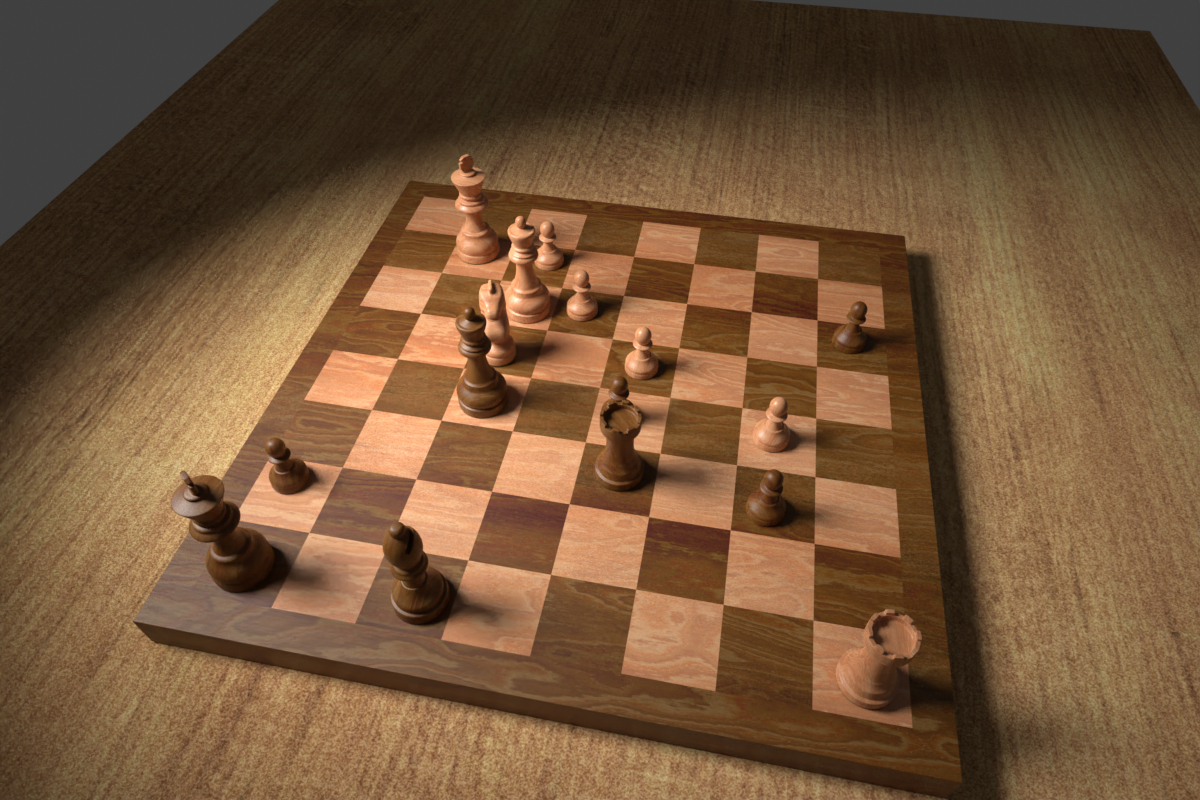
\includegraphics[width=0.8\linewidth]{fig/treino.jpg}
  \caption{Exemplo de Treino (Dataset \ref{osf})}
\label{fig:treino}
\end{figure}

O Dataset \ref{MYM} provavelmente será utilizado apenas na etapa de avaliação do programa,
aliado de outras figuras obtidas na internet e fotografadas pelos próprios projetistas.
Os Datasets 1 e 2 já são estão com suas bounding boxes anotadas e rotuladas.
O primeiro possui um arquivo em .csv para cada imagem,
com informações detalhadas sobre as características com que o 3d foi elaborado.

Já o segundo é obtido a partir do RoboFlow, que permite download dos detalhes em diversos formatos.
Roboflow é uma plataforma para machine learning que fornece gratuitamente alguns serviços como anotação de figuras,
\textit{data augmentation}, estatísticas sobre datasets, e até treinamento de modelos.
Provavelmente será utilizada na anotação de figuras não-rotuladas.
Além disso, será necessário unificar o formato de anotação entre os datasets.
Caso não seja encontrado um código pronto para estas conversões, os alunos criarão um algoritmo para tal.

Ainda existe a possibilidade de obter mais datasets através de aquisição de fotos
não rotuladas da internet ou dos próprios alunos, e usar técnicas de \textit{data augmentation}
E rotular essas imagens manualmente 
(com o auxílio do RoboFlow ou algum sistema otimizado desenvolvido pelos alunos).

\subsubsection{Reconhecimento}

Com os datasets analisados e organizados, é hora de treinar o modelo.
Diversas condições de treinamento serão avaliadas, priorizando aquelas já abordadas pela literatura.
Com um modelo treinado, será possível fornecer imagens para avaliação.

A detecção e reconhecimento das peças se dará por meio do TensorFlow e suas APIs.
No início, a imagem (filtrada) será encaminhada ao TensorFlow Object Detection que detectará as features na figura.
Com as coordenadas das caixas delimitadores,
as peças serão selecionadas e avaliadas no modelo, obtendo-se assim, a melhor estimativa para o rótulo daquela imagem.

\begin{figure}[h!]
\centering
  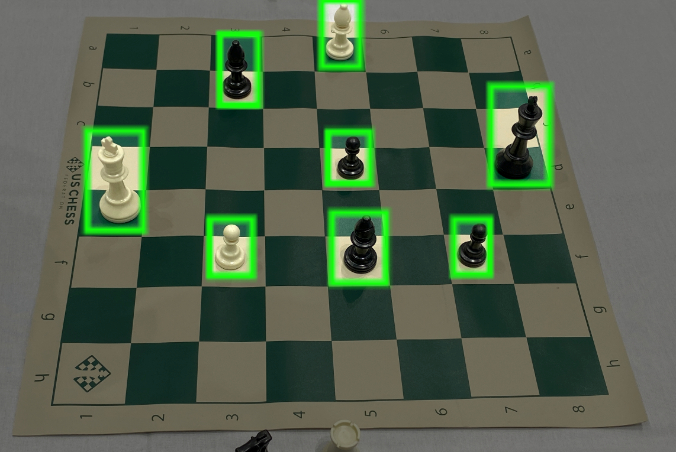
\includegraphics[width=0.7\linewidth]{fig/delimitar.jpg}
  \caption{Exemplo de caixas de delimitação nas peças (Dataset \ref{roboflow})}
\label{fig:delimitar}
\end{figure}

\subsection{Integração entre as ferramentas e possibilidades}

A integração entre o mundo de inteligência artificial e visão computacional é uma etapa crucial deste projeto.
Ela permitirá indicar em qual posição do tabuleiro cada uma das peças detectadas pelo TensorFlow pertence.
Aqui, o conteúdo das caixas delimitadoras será segmentado com uso de computação visual, separando a peça do tabuleiro.

Com apenas a área da peça em mãos,
é possível verificar com qual casa há maior intersecção desta (por produto interno, por exemplo).
Por que segmentar as peças, e não utilizar apenas a caixa como um todo?
Pois de acordo com o ângulo no qual o tabuleiro se encontra,
a maior parte da caixa pode ocupar outra posição, o que reduziria drasticamente a eficácia.

De acordo com cor das casas nas ``esquinas" do tabuleiro,
é possível saber a direção onde os jogadores estão posicionados,
porém muitas vezes não é possível aferir com certeza de qual lado cada um está baseado unicamente na distribuição das peças.
Portanto, este projeto se propõe a fornecer duas posições considerando as duas possibilidades
(lado das pretas e lado das brancas).
Outras possibilidades para esse problema são:
Restringir o usuário do sistema a utilizar fotos somente de um mesmo lado do tabuleiro,
ou utilizar um software de avaliação de posição para determinar a posição mais provável
(posições com grande vantagem para um jogador são mais improváveis).

\section{Ferramentas}
Este projeto será desenvolvido na linguagem Python em Jupyter Notebooks,
com o auxílio de diversas bibliotecas, principalmente:
TensonFlow, Keras, OpenCV, Scikit-Image, Pandas, Matplotlib, entre outras.

Para maior comodidade nos testes e garantia de cumprimento do prazo,
os alunos se propõem a investir em acesso a computação em nuvem se necessário.
Até o momento, a plataforma Google Cloud se mostrou mais atrativa por conceder 300 dólares de crédito para novos usuários,
mas outras soluções poderão ser adotadas.

\section{Projetos semelhantes}
Durante a quarentena, a busca por xadrez aumentou vertiginosamente,
este aumento de interesse se manifestou também nos desenvolvedores.
Foram encontrados alguns projetos semelhantes ao nosso na internet.
O mais interessante foi o de Maciej A. Czyzewski, Artur Laskowski, e Szymon Wasik.
O algoritmo por eles desenvolvido obteve bons resultados:
\cite{czy20}:
\blockquote{The described method performs extraordinarily well and achieves an accuracy over
            99.5\% for detecting chessboard lattice points (compared to the 74\% for the best alternative),
            95\% (compared to 60\% for the best alternative) for positioning the chessboard in an image, and almost
            95\% for chess piece recognition. (CZYZEWSKI; LASKOWSKI; WASIK; 2020)}

A abordagem deles consiste em usar um mapa de calor para determinar a localização do tabuleiro na foto,
detecção de linhas retas, algoritmo de determinação dos vértices, e uso de rede neural para reconhecer as peças.

A maioria dos outros projetos semelhantes utilizaram datasets de apenas um tabuleiro,
a proposta deste projeto é criar um modelo para auxiliar no reconhecimento de qualquer tabuleiro de xadrez.
Além disso, nenhum dos projetos que se propôs a identificar fotografias de tabuleiros foi implementado com TensorFlow
(maioria usou PyTorch).
Outros programas também foram utilizados com foco em imagens de tabuleiros online ou de livros de xadrez,
que pode auxiliar o desenvolvimento do algoritmo.

\section{Avaliação do Modelo}
O modelo será avaliado de acordo com a acurácia,
serão analisadas as matrizes confusão de cada peça e é possível também gerar um
heatmap com a matriz de probabilidades de engano entre as peças.
Neste sentido, também se buscará ter uma noção para cada tipo de peça fazendo o uso de sua matriz confusão.
Outra ferramenta utilizada será a matriz de correlação das probabilidades.

\nocite{*}
\printbibliography
\end{document}
